\documentclass[12pt]{article}

\usepackage{sbc-template}

\usepackage{graphicx,url}

% For Brazilian portuguese language
\usepackage[utf8]{inputenc}
\usepackage[brazil]{babel}
     
\sloppy

\title{Aplicativo de Troca de Mensagens Utilizando Criptografia Baseada em
Imagens}

\author{Marcus Antonio Grécia Brandt\inst{1}, Mikhail Yasha Ramalho \inst{1}}

\address{
Centro de Ensino Superior FUCAPI (CESF)\\Av. Gov. Danilo de Mattos Areosa, 381 -- Distrito Industrial -- Manaus -- AM -- Brasil
\email{\{marcusbrandt, mikhailramalho\}@gmail.com}
}

\begin{document} 

\maketitle

\begin{abstract}
  This meta-paper describes the style to be used in articles and short papers
  for SBC conferences. For papers in English, you should add just an abstract
  while for the papers in Portuguese, we also ask for an abstract in
  Portuguese (``resumo''). In both cases, abstracts should not have more than
  10 lines and must be in the first page of the paper.
\end{abstract}
     
\begin{resumo} 
  Aplicações de troca de mensagens possuem naturalmente um forte apelo popular
  e figuram como aplicações de destaque nas lojas de aplicativos. Porém levantam
  questões relativas a segurança e confiabilidade das informações que por eles
  trafegam. Este artigo descreve a implementação de um aplicativo de comunicação
  por meio do bluetooth que utiliza um algoritmo de criptografia baseado em
  imagens como chave de acesso.
\end{resumo}

\section{Introdução}

\section{Fundamentação Teórica} \label{sec:fundamentacao}

\subsection{ASCII}
O ASCII \textit{American Standard Code for Information Interchange} (Código Padrão Americano Para o Intercâmbio de Infromação) é um esquema de codificação inicialmente baseado no alfabeto americano, posteriormente se tornou um esforço para padronização da representação de caracteres pelos fabricantes de computadores.

Cada caracter (pontuação, valores alfanuméricos e valores de controle) é representado por um valor numérico divididos em uma tabela. Originalmente como eram representados apenas caracters americanos, acentuações e letras com essa característica não podiam ser representados, posteriormente a tabela passou por uma revisão e foram criadas 12 novas partes pra suprir essa necessidade.

\subsection{Imagem}
Quando digitalizadas as imagens são representadas por bits e bytes que são convertidos para números pra representar cada cor de um pixel específico, podendo ser representada por uma matriz de pixels(Figura~\ref{fig:repImage}) .  

\begin{figure}[ht]
\centering
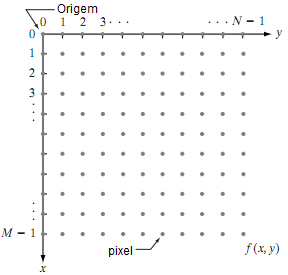
\includegraphics[width=.3\textwidth]{images/image.png}
\caption{Representação de uma imagem digital}
\label{fig:repImage}
\end{figure}

\subsection{Criptografia}
Criptografia é o estudo de técnicas pela qual as informações podem ser trocadas de forma segura através de um canal de comunicação aberto, tornando a mensagem em algo conhecido apenas pelos seus agentes.
\subsubsection{Chave Simétrica}
No processo de criptografia simétrica existe uma chave que é compartilhada entre todos os que pretendem desenciptar a mensagem, essa é a principal desvantagem desse método pois assumimos que todos que se utilizam da chave poderam obter as informações relacionadas a criptografia da mensagem, outro problema é o gerenciamento das chaves, olhando por um cenário de uma empresa todos que utilizar chaves que permitissem acesso a informações específicas tornando o gerenciamento das chaves problemático (Figura~\ref{fig:simProc}).


O processo de criptografia simétrica pode se dar por duas formas substituição e cifra de transposição (ou blocos), ambos podem ser bit-a-bit ou bloco de dados.

\begin{figure}[ht]
\centering
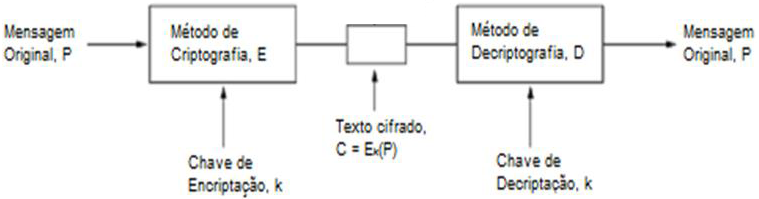
\includegraphics[width=.7\textwidth]{images/process_sim.png}
\caption{Sistema Criptográfico de Chave Simétrica} \cite{mikhail:2010}
\label{fig:simProc}
\end{figure}

\subsubsection{Chave Assimétrica}

No processo de criptografia assimétrica existem duas chaves diferentes mas matematicamente relacionadas para criptografar e descriptografar, são conhecidas como chave pública e chave privada, a chave pública pode ser distribuída para todas as outras partes para o processo de criptografia e a informação só poderá ser desencriptada com a chave privada (Figura~\ref{fig:simProc}) e essa é a principal diferença entre os dois métodos.

\begin{figure}[ht]
\centering
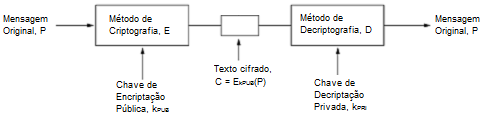
\includegraphics[width=.7\textwidth]{images/process_assim.png}
\caption{Sistema Criptográfico de Chave Assimétrica} \cite{mikhail:2010}
\label{fig:assimProc}
\end{figure}

\subsection{Bluetooth}
Bluetooth é uma tecnologia sem fio para troca de informação em pequenas distâncias baseada em ondas curtas e é padronizada pelo IEEE 802.15.1, foi originalmente concebida para ser alternativa ao RS-232. 

Ele opera em uma faixa de freqência de 2400–2483.5 MHz, utiliza a tecnoligia de rádio chamada de salto de frêquencia em espalhamento espectral (\textit{frequency-hopping spread spectrum}). Baseado em um protocolo de troca de pacotes com estrutura de \textit{master-slave}.

Um servidor Bluetooth pode se comunicar com até 7 devices em uma rede piconet (\textit{ad-hoc}) baseada na tecnologia Bluetooth.
\section{Sistema}
\subsection{Android}
O protótipo apresentado neste trabalho foi desenvolvido em Android, por ser uma plataforma popular para desenvolvimento de aplicativos móveis. O Android possui interfaces de programação de aplicativo (APIs), que vêm com o seu Software Development Kit (SDK) e possui recursos completos de interface\cite{android:2014}.

Para este protótipo utilizamos a versão 4.4.2 do Android conhecida como Jelly Beans, por ser a versão mais recente disponível, quando do desenvolvimento deste trabalho. 
\subsection{OpenCV}
O OpenCV é um conjunto de bibliotecas desenvolvidas com o objetivo de provêr visão computacional em tempo real. Desenvolvida originalmente em C mudou sua plataforma para C++ com o objetivo de se tornar mais facil o desenvolvimento de novas funcionalidades, melhor implementação e aplicação de padrõee, com suporte em Python e Java (Android), com suporte em Windows, Linux, iOS, Mac OS e Android.
\subsection{Java \& JNI}
Java é uma linguagem de programação adotada como padrão no desenvolvimento de aplicativos em Android, é baseada em classes, orientada a objeto e exitem várias APIS (biblioteca) [qual o melhor?] prontas, oferecendo uma sintaxe muito parecida com C e C++ é atualmente a linguagem mais popular do mundo utilizada principalmente em sistemas web cliente-servidor, foi originalmente desenvolvida por James Gosling na Sun Microsystems porteriormente adquirida pela Oracle.

Para comunicações mais baixo nível o java utiliza um artificio de comunicação via callbacks através da sua api de comunicação nativa a JNI (\textit{Java Native Interface})
\subsection{Processo de Criptografia}
\subsection{Sistema de Criptografia Utilizando Imagens}
Nossa proposta é composta primeiramente por um algoritmo de chave simétrica, pois haverá uma troca de cada caracter por uma correspondente da imagem escolhida. O processo de criptografia que utilizamos nesse artigo proposto por \cite{mikhail:2010} consistem em utilizar uma imagem como chave para encriptação (Figura~\ref{fig:encFig}) e para desencriptação (Figura~\ref{fig:decFig}). O algoritmo se baseia na seguinte ideia:

*Uma imagem é representada por pixels que tem valores de 0 até 255 assim como a tabela ASCII que tem valores de 0 à 255 incluindo digítos de controle.

*Um problema pode ocorrer na substituição de alguns caracters quando não houver correspondente na imagem. Podendo tornar o custo do algoritmo maior.
\begin{figure}[ht]
\centering
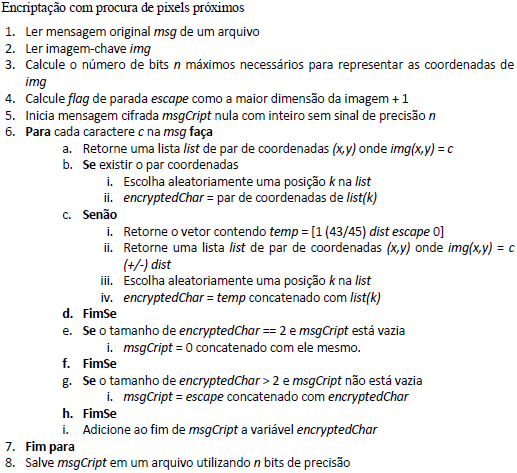
\includegraphics[width=.9\textwidth]{images/process_encrypt.png}
\caption{Algoritmo de encriptação  \cite{mikhail:2010}}
\label{fig:encFig}
\end{figure}

*Será utilizada a mesma imagem para decriptografia do mesmo.

*Havendo caracteres sendo representados pelos mais próximos calcularemos o valor real para desencriptar.

\begin{figure}[ht]
\centering
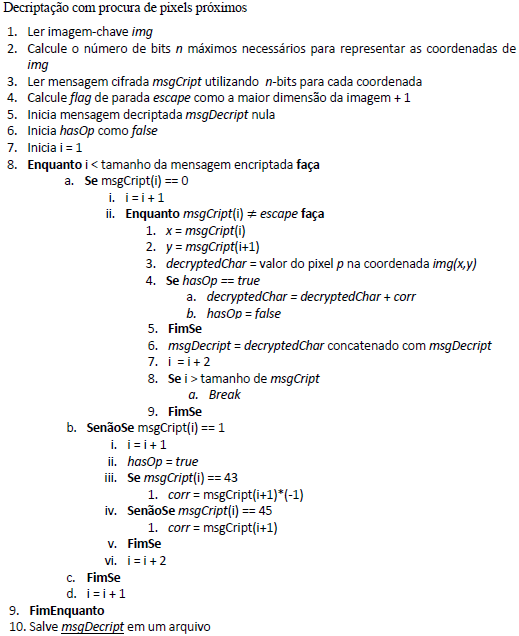
\includegraphics[width=.9\textwidth]{images/process_decrypt.png}
\caption{Algoritmo de desencriptação \cite{mikhail:2010}}
\label{fig:decFig}
\end{figure}

\section{Resultados}\label{sec:resultados}
\section{Conclusão}\label{sec:conclusao}


\bibliographystyle{sbc}
\bibliography{sbc-template}
\end{document}
